\documentclass{article}

\usepackage{color}
\usepackage{graphicx}
\usepackage{amsmath}
\usepackage{bm}
\usepackage{enumerate}
\usepackage{booktabs}
\usepackage{cite}
\usepackage{geometry}
\usepackage{url}
\usepackage{float}
\usepackage{indentfirst}
\usepackage{ulem}
\usepackage{multirow}
\begin{document}

\vspace*{0.25cm}

\noindent\hrulefill

\thispagestyle{empty}

\begin{center}
    \begin{large}
        \sc{UM--SJTU Joint Institute \vspace{0.3em} \\ Introduction to Circuits \\(Ve215)}
    \end{large}

    \hrulefill

    \vspace*{5cm}
    \begin{Large}
        \sc{{Laboratory Report}}
    \end{Large}

    \vspace{2em}

    \begin{large}
        \sc{{Lab 4
                    \vspace{0.5em}

                    AC Lab}}
    \end{large}
\end{center}
\vfill

\begin{table}[h!]
    \flushleft
    \begin{tabular}{ll}
        Name: Kang Jiaming \hspace*{2em} &
        ID: 518021911220 \hspace*{2em}     \\

        \\

        Date:  6 Nov. 2019
    \end{tabular}
\end{table}

\hfill
\newpage

\section{Goals\label{goals}}
\noindent The goals for this lab are:
\begin{enumerate}
    \item Learn how to define, calculate, and measure the amplitude of a sinusoidal signal.
    \item Learn how to define, calculate, and measure the Rise Time and Fall Time of a signal.
    \item Learn how to observe FFT spectra of signal and measure their parameters with cursors.
    \item Measure the waveforms and FFT spectra of various signals.
    \item Compare your theoretical results obtained in the Pre-Lab with your In-Lab data.
\end{enumerate}

\section{Introduction\label{intro}}

\subsection{High-Z mode}

You have already learnt Thevenin equivalent of a circuit. You can think the function generator in terms of its Thevenin equivalent circuit, which includes the voltage source and $V_S$ and the equivalent resistance of $50\Omega$ as shown below.

\begin{figure}[H]\centering
    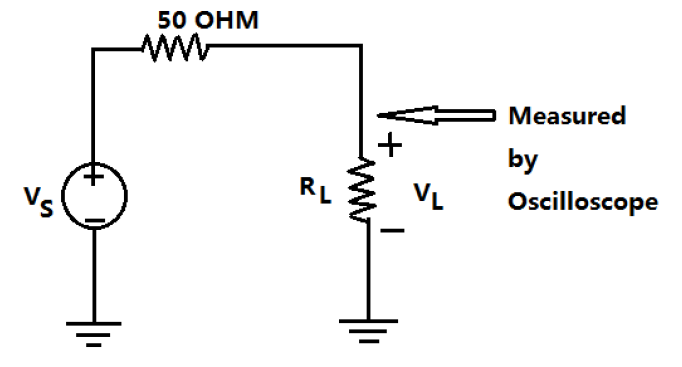
\includegraphics[scale=1.0]{highz.png}
    \caption{Thevenin equivalent circuit of the function generator.}
\end{figure}

When the load $R_L$ is $50\Omega$, according to voltage division, we know that the $V_L$ measured will be $0.5V_S$. In this case, we use the 50 OHM mode, in which the function generator produces voltage $V_S$ but displays voltage $0.5V_S$. In that way, if you set $2V_{ppk}$ for the function generator, the actual $V_S$ will be $4V_{ppk}$ to make sure the load get a voltage of $2V_{ppk}$.

In our lab measurements, the load resistance $R_L$ is very high-the input resistance of the oscilloscope is about $1M\Omega$. The $V_L$ measured across $R_L$ practically equals $V_S$. So we use High Z mode, in which the function generator produce voltage $V_S$ and displays $V_S$.

\subsection{The Rise Time and Fall Time of signals}

The Rise time is the interval between the moment of the time when the signal reaches its $10\%$ level and the moment of time when the signal reaches its $90\%$. We have already used this concept in our Lab3.

\begin{figure}[H]\centering
    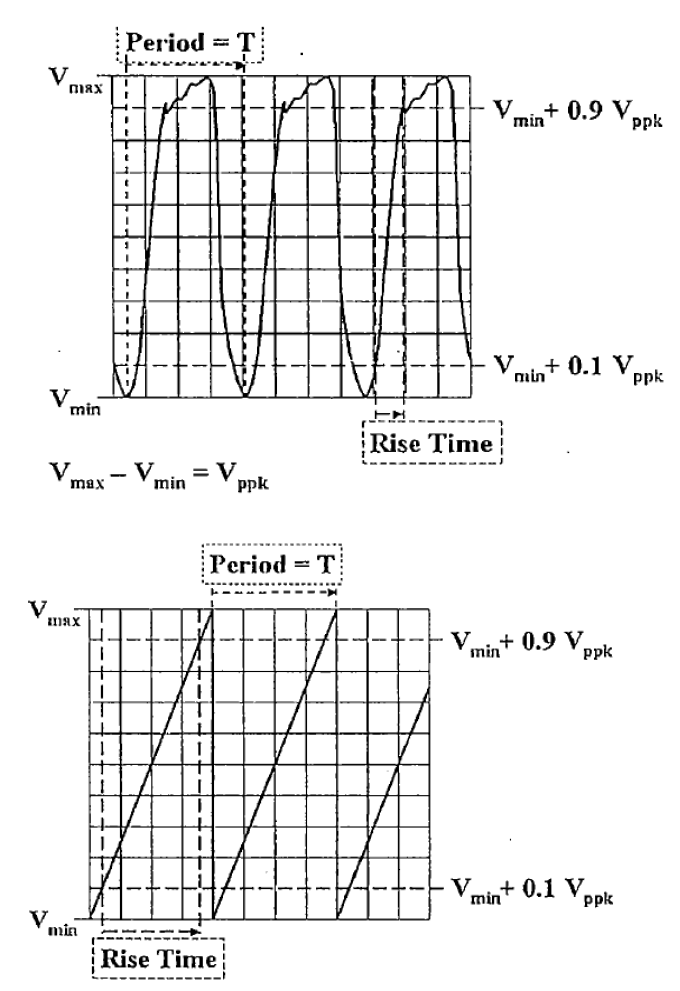
\includegraphics[scale=1.0]{rise.png}
    \caption{Rise time of a saw-tooth and a sinusoidal like wave.}
\end{figure}

The above two figures illustrate the rise time of a sinusoidal like wave and a saw-tooth wave. If you do not know what is $V_{ppk}$, you can refer to part 4 of this section.

Take the sinusoid wave as an example to calculate the rise time.
$$y = \frac{V_{ppk}}{2}\sin(2\pi ft)$$
$$V_{min} = -\frac{V_{ppk}}{2}, V_{max} = -\frac{V_{ppk}}{2}$$
$$RiseTime = \frac{\sin^{-1}\big(\frac{V_{min}+0.9V_{ppk}}{0.5V_{ppk}}\big)-\sin^{-1}\big(\frac{V_{min}+0.1V_{ppk}}{0.5V_{ppk}}\big)}{2\pi f}$$

\subsection{Fourier Series Representation of a Signal}

Fourier series is a way to represent a wave-like function as a combination of simply sine waves. It decomposed and period function into the sum of a (possibly infinite) set of simple oscillation functions.

Let $x(t)$ be a periodic signal with fundamental period $T_0$. It can be represent by the following synthesis equation,
$$x(t) = \sum^\infty_{k=-\infty}c_ke^{jk\omega_0t},$$
where $\omega_0=\frac{2\pi}{T_0}$. The coefficients $c_k$ in the above equation can be calculated by the analysis equation,
$$c_k = \frac{1}{T_0}\int^{T_0}_{0}x(t)e^{-jk\omega_0t}dt,\hspace{3em}k=0, \pm 1,...$$

\begin{figure}[H]\centering
    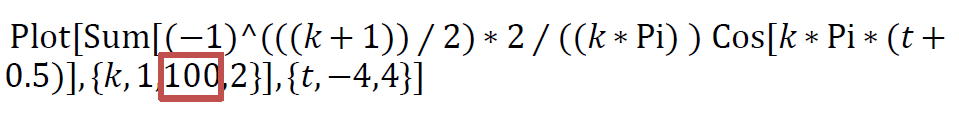
\includegraphics[scale=1.0]{code.png}
\end{figure}

You can use the above Mathematic code to get the feeling of how a series of
sinusoidal waves can form a square wave (actually, any waveform). You can
change the value in the red box, and the larger the value is, the more accurate the
result will be. Here we thank the Vv286 TA for FA2014 Gao Yuan for offering us the source
code.\\

For value 3, we can get the following result.
\begin{figure}[H]\centering
    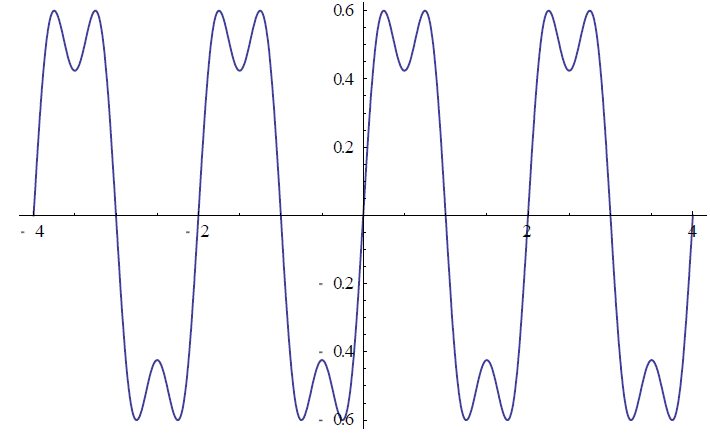
\includegraphics[scale=1.0]{value3.png}
\end{figure}
For value 20, we can get the following result,
\begin{figure}[H]\centering
    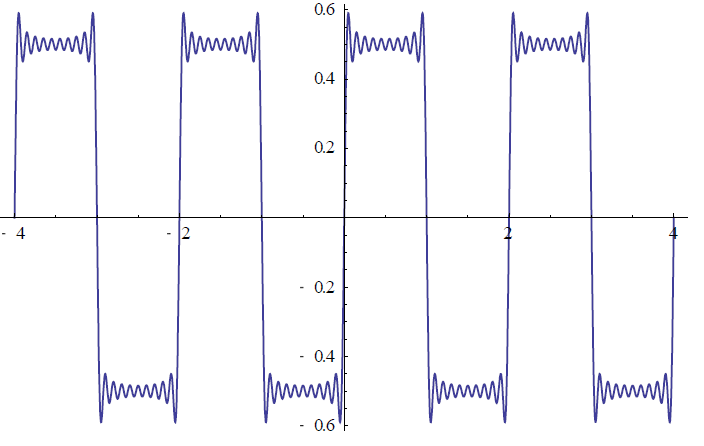
\includegraphics[scale=1.0]{value20.png}
\end{figure}
And for value 100, we get,
\begin{figure}[H]\centering
    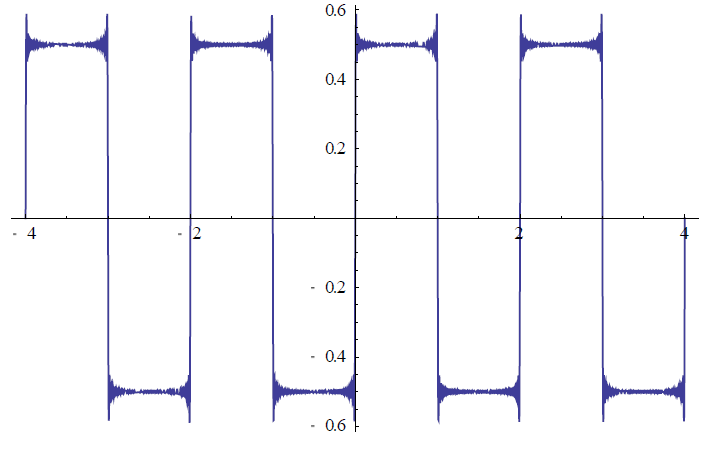
\includegraphics[scale=1.0]{value100.png}
\end{figure}

\subsection{Four ways to measure the amplitude of a sinusoid}
\begin{enumerate}[a)]
    \item $V_{peak}=V_p=V_{pk}=V_0$ is the peak amplitude of the sinusoid measured in V or mV.
    \item $V_{peak-to-peak}=V_{ppk}=V_{max}-V_{min}=2V_0$ is the value we often use in the lab to determine the overall size of the waveform. We have used it many times in the previous Labs.
    \item $V_{RMS}$ is the Root-Mean-Square, or RMS amplitude of the sinusoid. The sinusoidal voltage $V = V_0\sin(\omega t+\theta)$ dissipates as much power in the load resistor as does the DC voltage equals to $V_{RMS}$.

          \begin{figure}[H]\centering
              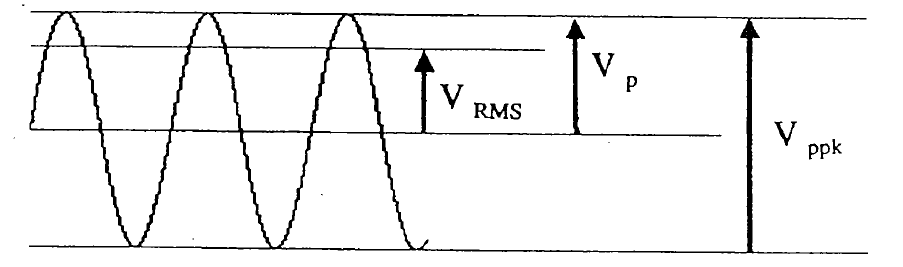
\includegraphics[scale=1.0]{V.png}
              \caption{Different ways to measure the amplitude of a sinusoid.}
          \end{figure}

          For any periodic function $f(t)$ that has period $T$, the RMS amplitude is defined as
          $$Amplitude, RMS = \sqrt{\frac{1}{T}\int^{t_0+T}_{t_0}f^2(t)dt}.$$
          In the case of sinusoid $f(t) = V_0\sin(\omega t+\theta)$.
          $$V_{RMS} = \frac{V_0}{\sqrt{2}} = \frac{V_{peak}}{\sqrt{2}} = \frac{V_{ppk}}{2\sqrt{2}}.$$
    \item The above three ways all study the signal in time domain, plotted as voltage vs. time. In this Lab, we also need to study the frequency domain, when you measure their spectra displayed as amplitude vs. frequency. In frequency domain, the oscilloscope measures the amplitude of on a logarithmic scale, using decibels.
          $$dBV = 20\log_{10}\bigg(\frac{Amplitude\,\,in\,\,V_{RMS}}{1V_{RMS}}\bigg).$$
          Decibels are used to calculate ratios of two amplitudes on a logarithmic scale.
          $$Ratio, in dB = 20\log_{10}\bigg(\frac{Amplitude\,\,of\,\,signal\,\,\#2,RMS}{Amplitude\,\,of signal\,\,\#1,RMS}\bigg).$$
\end{enumerate}

\section{Results}

\subsection{Part I}

The data are shown in Table \ref{Table1}.

\begin{table}[H]
    \centering
    \begin{tabular}{lcc}
        \toprule
                                  & Set on Function Generator & Measured with Oscilloscope \\
        \midrule
        Amplitude in $V_{pp}$ [V] & 3.000                     & 3.04                       \\
        Frequency [kHz]           & 1.000000                  & 1.00                       \\
        Rise Time [$\mu\text{s}$] & 295                       & 300                        \\
        \midrule
        Amplitude in $V_{pp}$ [V] & 5.000                     & 5.000                      \\
        Frequency [kHz]           & 1.500000                  & 1.49                       \\
        Rise Time [$\mu\text{s}$] & 197/                      & 190                        \\
        \bottomrule
    \end{tabular}
    \caption{Rise time measurement.}\label{Table1}
\end{table}

The theoretical rise time for $3V_{ppk}$, 1 kHz is
\begin{align*}
    Rise\,\,Time & = \frac{\sin^{-1}\big(\frac{V_{min}+0.9V_{ppk}}{0.5V_{ppk}}\big)-\sin^{-1}\big(\frac{V_{min}+0.1V_{ppk}}{0.5V_{ppk}}\big)}{2\pi f}         \\
                 & = \frac{\sin^{-1}\big(\frac{-1.5+0.9\times 3}{0.5\times 3}\big)-\sin^{-1}\big(\frac{-1.5+0.1\times 3}{0.5\times 3}\big)}{2\pi \times 1000} \\
                 & = 295\,\,[\mu\text{s}].
\end{align*}

The relative error is
$$\epsilon = \frac {300-295}{295}\times 100\% = 1.7\%.$$

\vspace*{0.3cm}

The theoretical rise time for $5V_{ppk}$, 1.5 kHz is
\begin{align*}
    Rise\,\,Time & = \frac{\sin^{-1}\big(\frac{V_{min}+0.9V_{ppk}}{0.5V_{ppk}}\big)-\sin^{-1}\big(\frac{V_{min}+0.1V_{ppk}}{0.5V_{ppk}}\big)}{2\pi f}         \\
                 & = \frac{\sin^{-1}\big(\frac{-2.5+0.9\times 5}{0.5\times 5}\big)-\sin^{-1}\big(\frac{-2.5+0.1\times 5}{0.5\times 5}\big)}{2\pi \times 1500} \\
                 & = 197\,\,[\mu\text{s}].
\end{align*}

The relative error is
$$\epsilon = \frac{197-190}{197}\times 100\% = 3.6\%.$$


\subsection{Part II}

\subsubsection{Wave with amplitude of 3 $V_{ppk}$ and frequency of 1 kHz}

The data measured for the sine wave at 3 $V_{ppk}$ and 1 kHz are shown in Table \ref{TableSine1}.

\begin{table}[H]\centering
    \begin{tabular}{ccc}
        \toprule
        Peak  & Frequency [kHz] & Amplitude [dBV] \\
        \midrule
        $f_0$ & 0.9600          & -1.60           \\
        \bottomrule
    \end{tabular}
    \caption{Data for the sine wave at 3 $V_{ppk}$ and 1 kHz.}\label{TableSine1}
\end{table}

The relative error of the frequency is
$$\epsilon_f = \frac{1-0.96}{1}\times 100\% = 4\%.$$

The theoretical amplitude in [dBV] is
$$V_{dBV} = 20\log_{10}\bigg(\frac{V_{ppk}}{2\sqrt{2}}\bigg) = 20\log_{10}\bigg(\frac{3}{2\sqrt{2}}\bigg) = 0.512\,\,[V].$$

The relative error of amplitude in [dBV] is
$$\epsilon_{V_{dBV}} = \frac{-0.512-(-1.60)}{0.512}\times 100\% = -412.5\%.$$

The data for the square wave at 3 $V_{ppk}$ and 1 kHz are shown in Table \ref{TableSquare1}.

\begin{table}[H]\centering
    \begin{tabular}{ccc}
        \toprule
        Peak   & Frequency [kHz] & Amplitude [dBV] \\
        \midrule
        $f_0$  & 1.000           & 0.00            \\
        $3f_0$ & 3.008           & -6.80           \\
        $5f_0$ & 5.000           & -10.0           \\
        $7f_0$ & 7.004           & -11.6           \\
        $9f_0$ & 9.016           & -12.4           \\
        \bottomrule
    \end{tabular}
    \caption{FFT spectrum for square wave.}\label{TableSquare1}
\end{table}

The Fourier series representation of a square wave with amplitude of 3 $V_{ppk}$ and frequency of 1 kHz is
$$f(t) = \frac{6}{\pi}\bigg(\sin(2\times10^3 \pi t) +\frac{1}{3}\sin(6\times10^3 \pi t) + \frac{1}{5}\sin(10\times10^3 \pi t) + \frac{1}{7}\sin(14\times10^3 \pi t) + \frac{1}{9}\sin(18\times10^3 \pi t) + \cdots\bigg).$$

According to the equation
$$V_{pk} = \sqrt{2}V_{RMS} = \sqrt{2}\cdot 10^{V_{dBV}/20}$$
and the method of Fourier series representation, we can calculate the measured and theoretical amplitude of the Fourier series representation of square wave in $V_{pk}$ and the frequency. The results and relative error are shown in Table \ref{TableSVppk1}.

\begin{table}[H]\centering
    \begin{tabular}{cccc}
        \toprule
        Peak   & Measured $V_{pk}$ [V] & Theoretical $V_{pk}$ [V] & relative error \\
        \midrule
        $f_0$  & 1.41                  & 1.91                     & 26 $\%$     \\
        3$f_0$ & 0.65                  & 0.64                     & 1 $\%$      \\
        5$f_0$ & 0.45                  & 0.38                     & 18 $\%$      \\
        7$f_0$ & 0.37                  & 0.28                     & 33 $\%$      \\
        9$f_0$ & 0.34                  & 0.21                     & 62 $\%$      \\
        \bottomrule
    \end{tabular}
    \caption{Measured and theoretical amplitude in $V_{pk}$ of the square wave.}\label{TableSVppk1}
\end{table}

\subsubsection{Wave with amplitude of 6 $V_{ppk}$ and frequency of 2 kHz}

The data measured for the sine wave at 6 $V_{ppk}$ and 2 kHz are shown in Table \ref{TableSine2}.

\begin{table}[H]\centering
    \begin{tabular}{ccc}
        \toprule
        Peak  & Frequency [kHz] & Amplitude [dBV] \\
        \midrule
        $f_0$ & 2.004           & 3.20            \\
        \bottomrule
    \end{tabular}
    \caption{Data for the sine wave at 6 $V_{ppk}$ and 2 kHz.}\label{TableSine2}
\end{table}

The relative error of the frequency is
$$\epsilon_f = \frac{2.004-2}{2}\times 100\% = 0.2\%.$$

The theoretical amplitude in [dBV] is
$$V_{dBV} = 20\log_{10}\bigg(\frac{V_{ppk}}{2\sqrt{2}}\bigg) = 20\log_{10}\bigg(\frac{6}{2\sqrt{2}}\bigg) = 6.53\,\,[V].$$

The relative error of the amplitude in [dBV] is
$$\epsilon_{V_{pk}} = \frac{3.20-6.53}{6.53}\times 100\% = -51.0\%.$$

The data for the square wave at 6 $V_{ppk}$ and 2 kHz are shown in Table \ref{TableSquare2}.

\begin{table}[H]\centering
    \begin{tabular}{ccc}
        \toprule
        Peak   & Frequency [kHz] & Amplitude [dBV] \\
        \midrule
        $f_0$  & 2.000           & 4.40            \\
        $3f_0$ & 4.000           & -14.8           \\
        $5f_0$ & 6.000           & -2.80           \\
        $7f_0$ & 8.000           & -14.0           \\
        $9f_0$ & 10.000          & -6.00           \\
        \bottomrule
    \end{tabular}
    \caption{FFT spectrum for square wave.}\label{TableSquare2}
\end{table}

The Fourier series representation of a square wave with amplitude of 6 $V_{ppk}$ and frequency of 2 kHz is
$$f(t) = \frac{12}{\pi}\bigg(\sin(4\times10^3 \pi t) +\frac{1}{3}\sin(12\times10^3 \pi t) + \frac{1}{5}\sin(20\times10^3 \pi t) + \frac{1}{7}\sin(28\times10^3 \pi t) + \frac{1}{9}\sin(36\times10^3 \pi t) + \cdots\bigg).$$

According to the equation
$$V_{pk} = \sqrt{2}V_{RMS} = \sqrt{2}\cdot 10^{V_{dBV}/20}$$
and the method of Fourier series representation, we can calculate the measured and theoretical amplitude of the Fourier series representation of square wave in $V_{pk}$ and the frequency. The results and relative error are shown in Table \ref{TableSVppk2}.

\begin{table}[H]\centering
    \begin{tabular}{cccc}
        \toprule
        Peak   & Measured $V_{pk}$ [V] & Theoretical $V_{pk}$ [V] & relative error \\
        \midrule
        $f_0$  & 3.60                  & 3.82                     & -39$\%$      \\
        3$f_0$ & 1.14                  & 1.27                     & -80$\%$     \\
        5$f_0$ & 0.69                  & 0.76                     & 35$\%$      \\
        7$f_0$ & 0.52                  & 0.55                     & -49$\%$      \\
        9$f_0$ & 0.42                  & 0.42                     & -69$\%$         \\
        \bottomrule
    \end{tabular}
    \caption{Measured and theoretical amplitude in $V_{pk}$ of the square wave.}\label{TableSVppk2}
\end{table}



\section{Conclusions and discussion}
In this lab, we get to know the concept of rise time and fall time, Fourier series representation and four different measures of amplitude. The amplitude, frequency, rise time of sine waves and square waves are measured. The experimental result is compared with the theoretical value. Fourier series are applied when calculating the theoretical value for square wave.

From the result section, it can be seen that the measurement of frequency is of relatively high accuracy, however the measurement of amplitude is of high error. Possible reasons may include the stability of the connection and the low precision of the apparatus. Also, the last three sets of data is obviously opposed to the theoretical trend. That is because the result is out of range when using the same scale, so we had to change the scale and thus the result are greatly affected.

\section{References}
\noindent [1] VE215 Lab4 AC Lab Manual

\section{Appendix}
\subsection{Photos}
The photos taken during the lab are attached below.
    
\begin{figure}\centering
    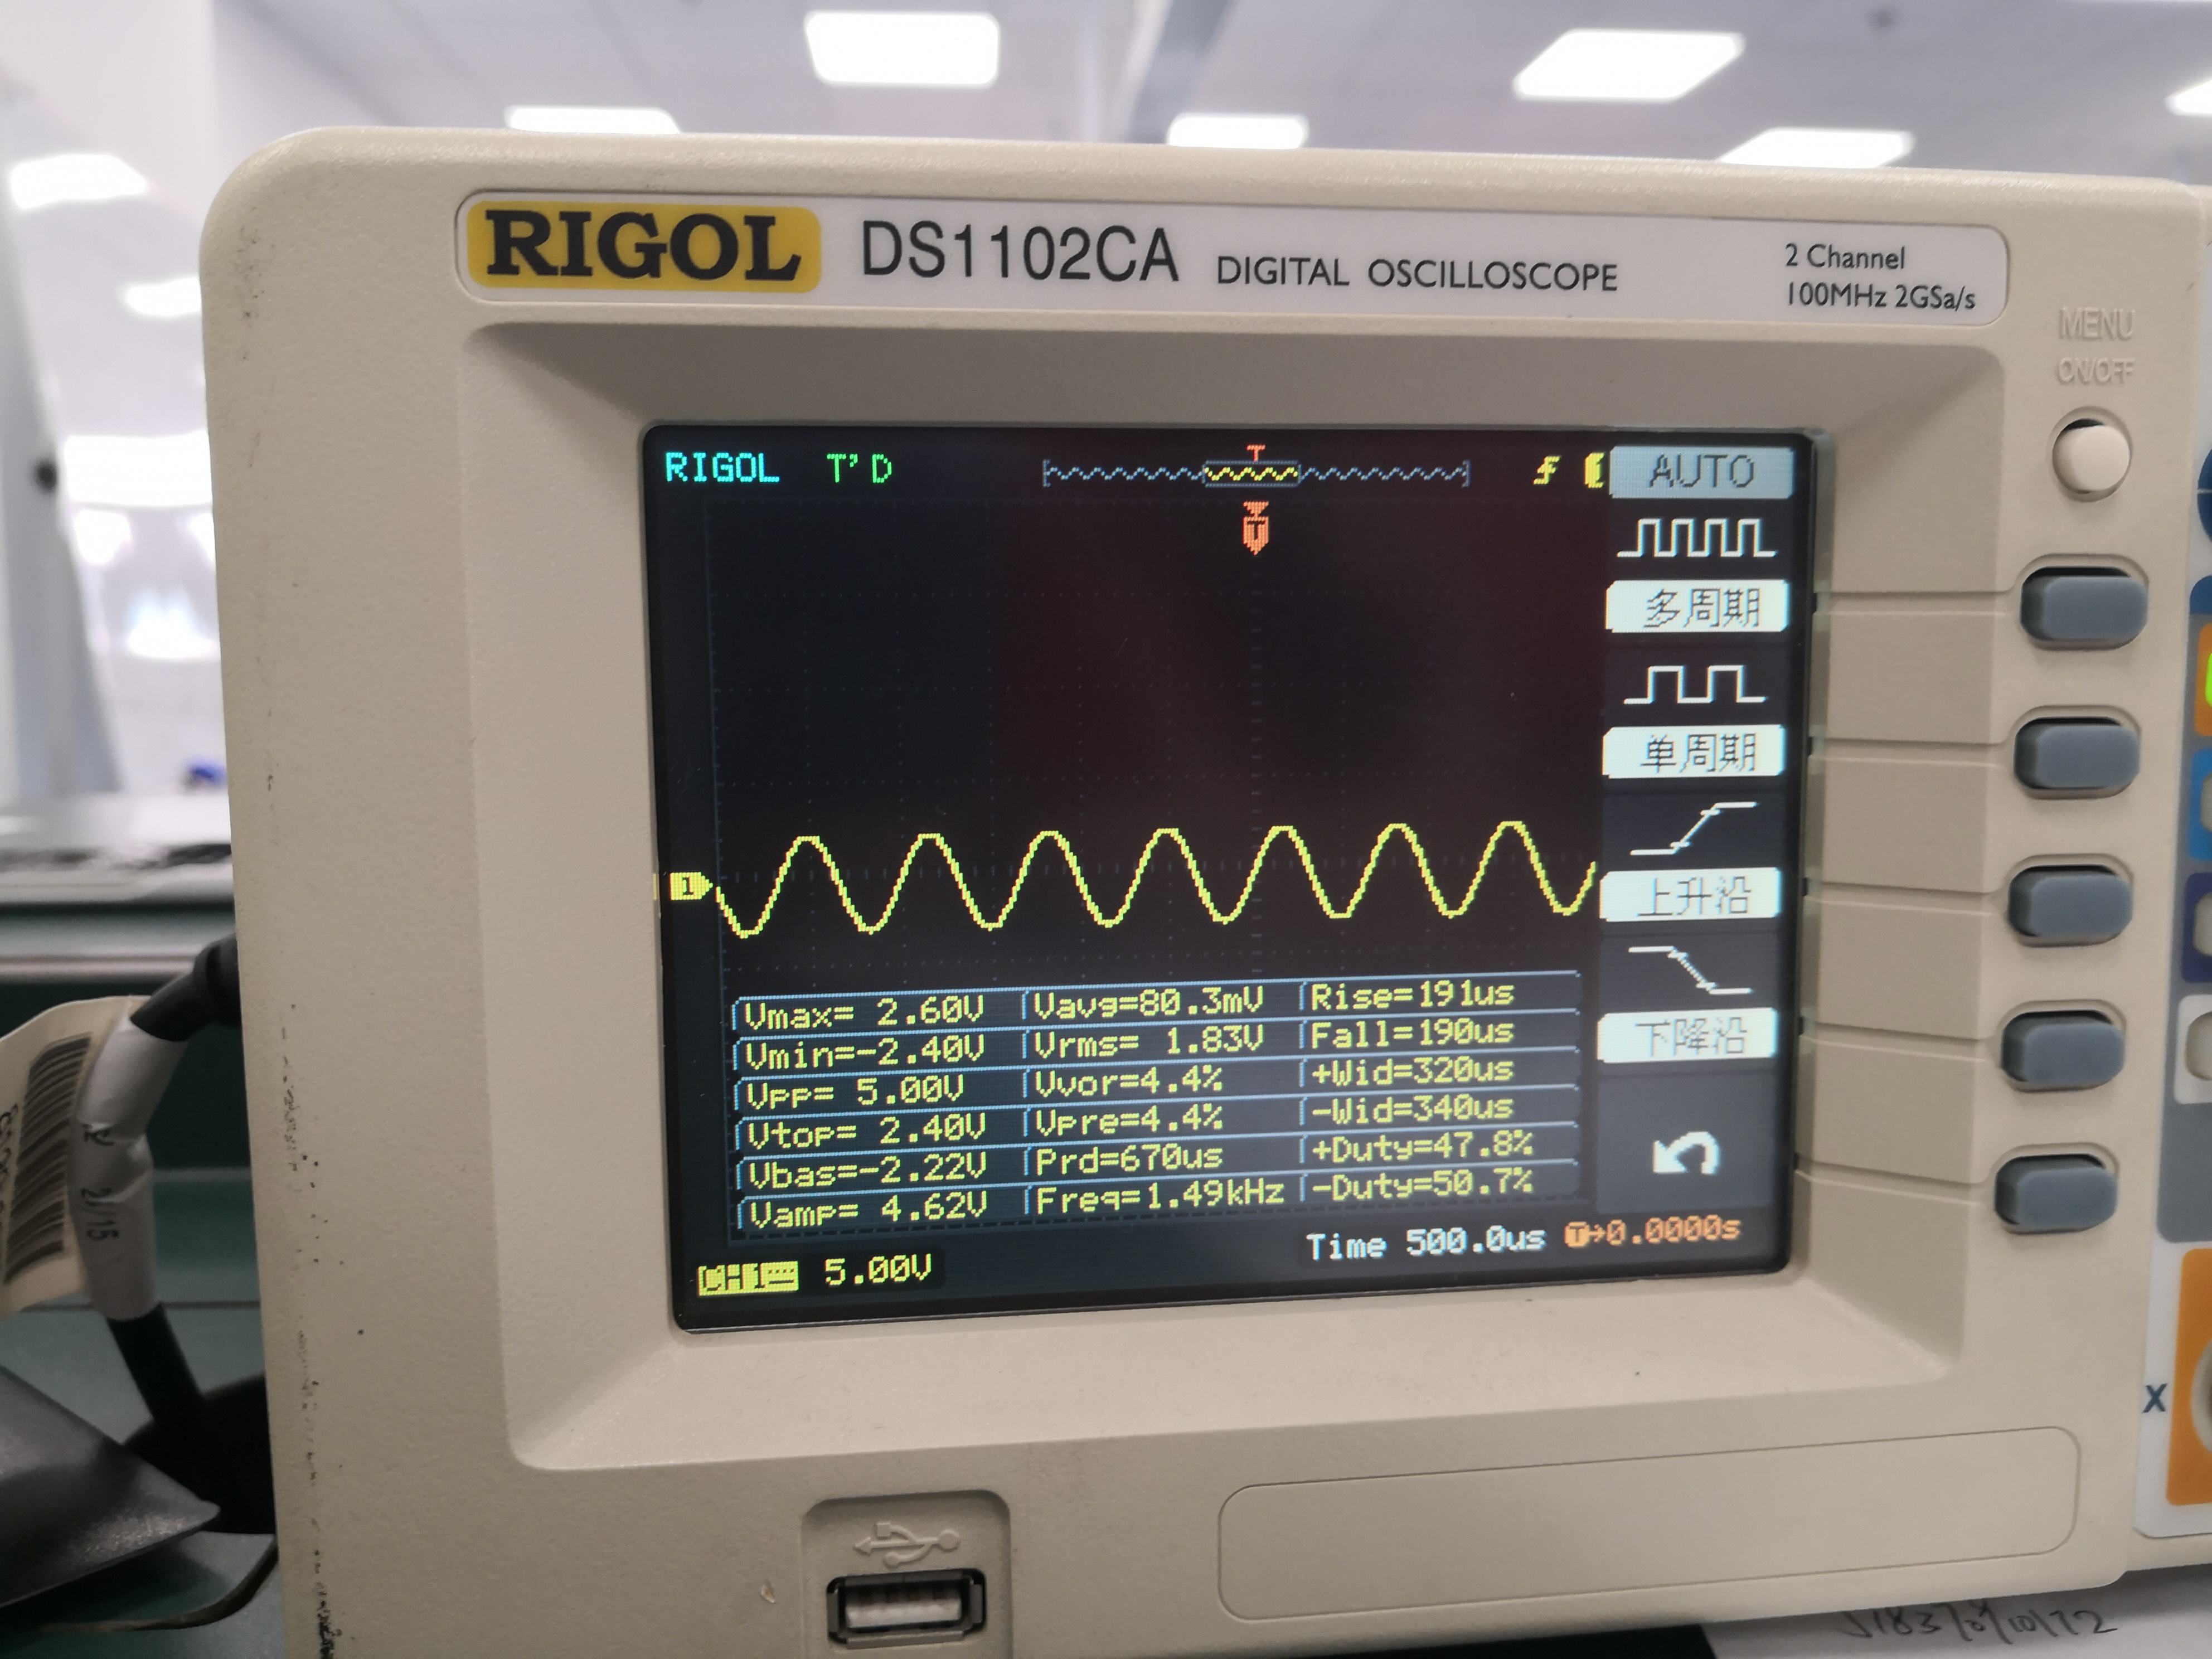
\includegraphics[width=0.45\textwidth]{1}
    
\end{figure}

\begin{figure}\centering
    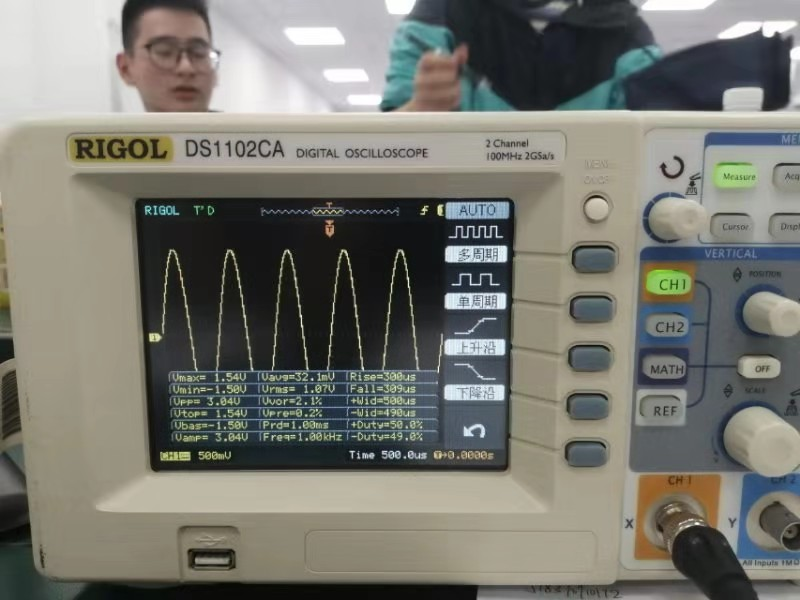
\includegraphics[width=0.45\textwidth]{2}
\end{figure}

\begin{figure}\centering
    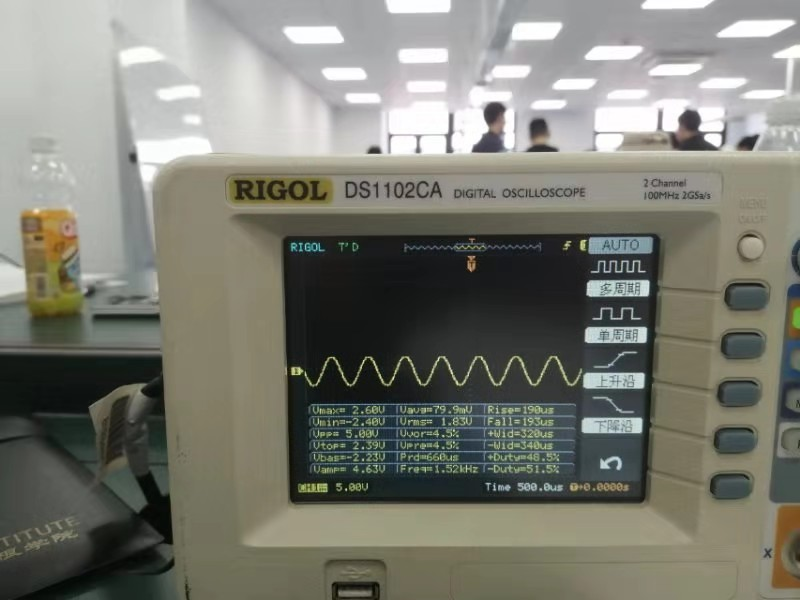
\includegraphics[width=0.45\textwidth]{3}
\end{figure}

\begin{figure}\centering
    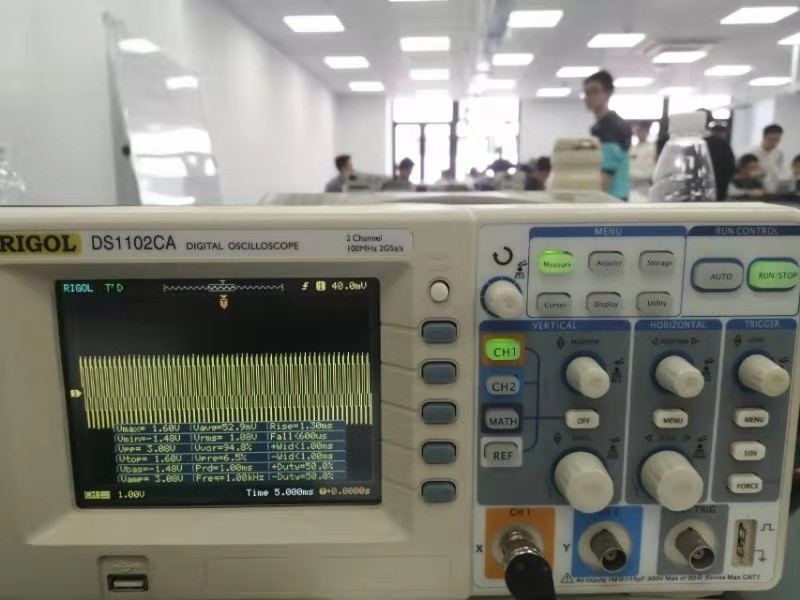
\includegraphics[width=0.45\textwidth]{4}
\end{figure}

\begin{figure}\centering
    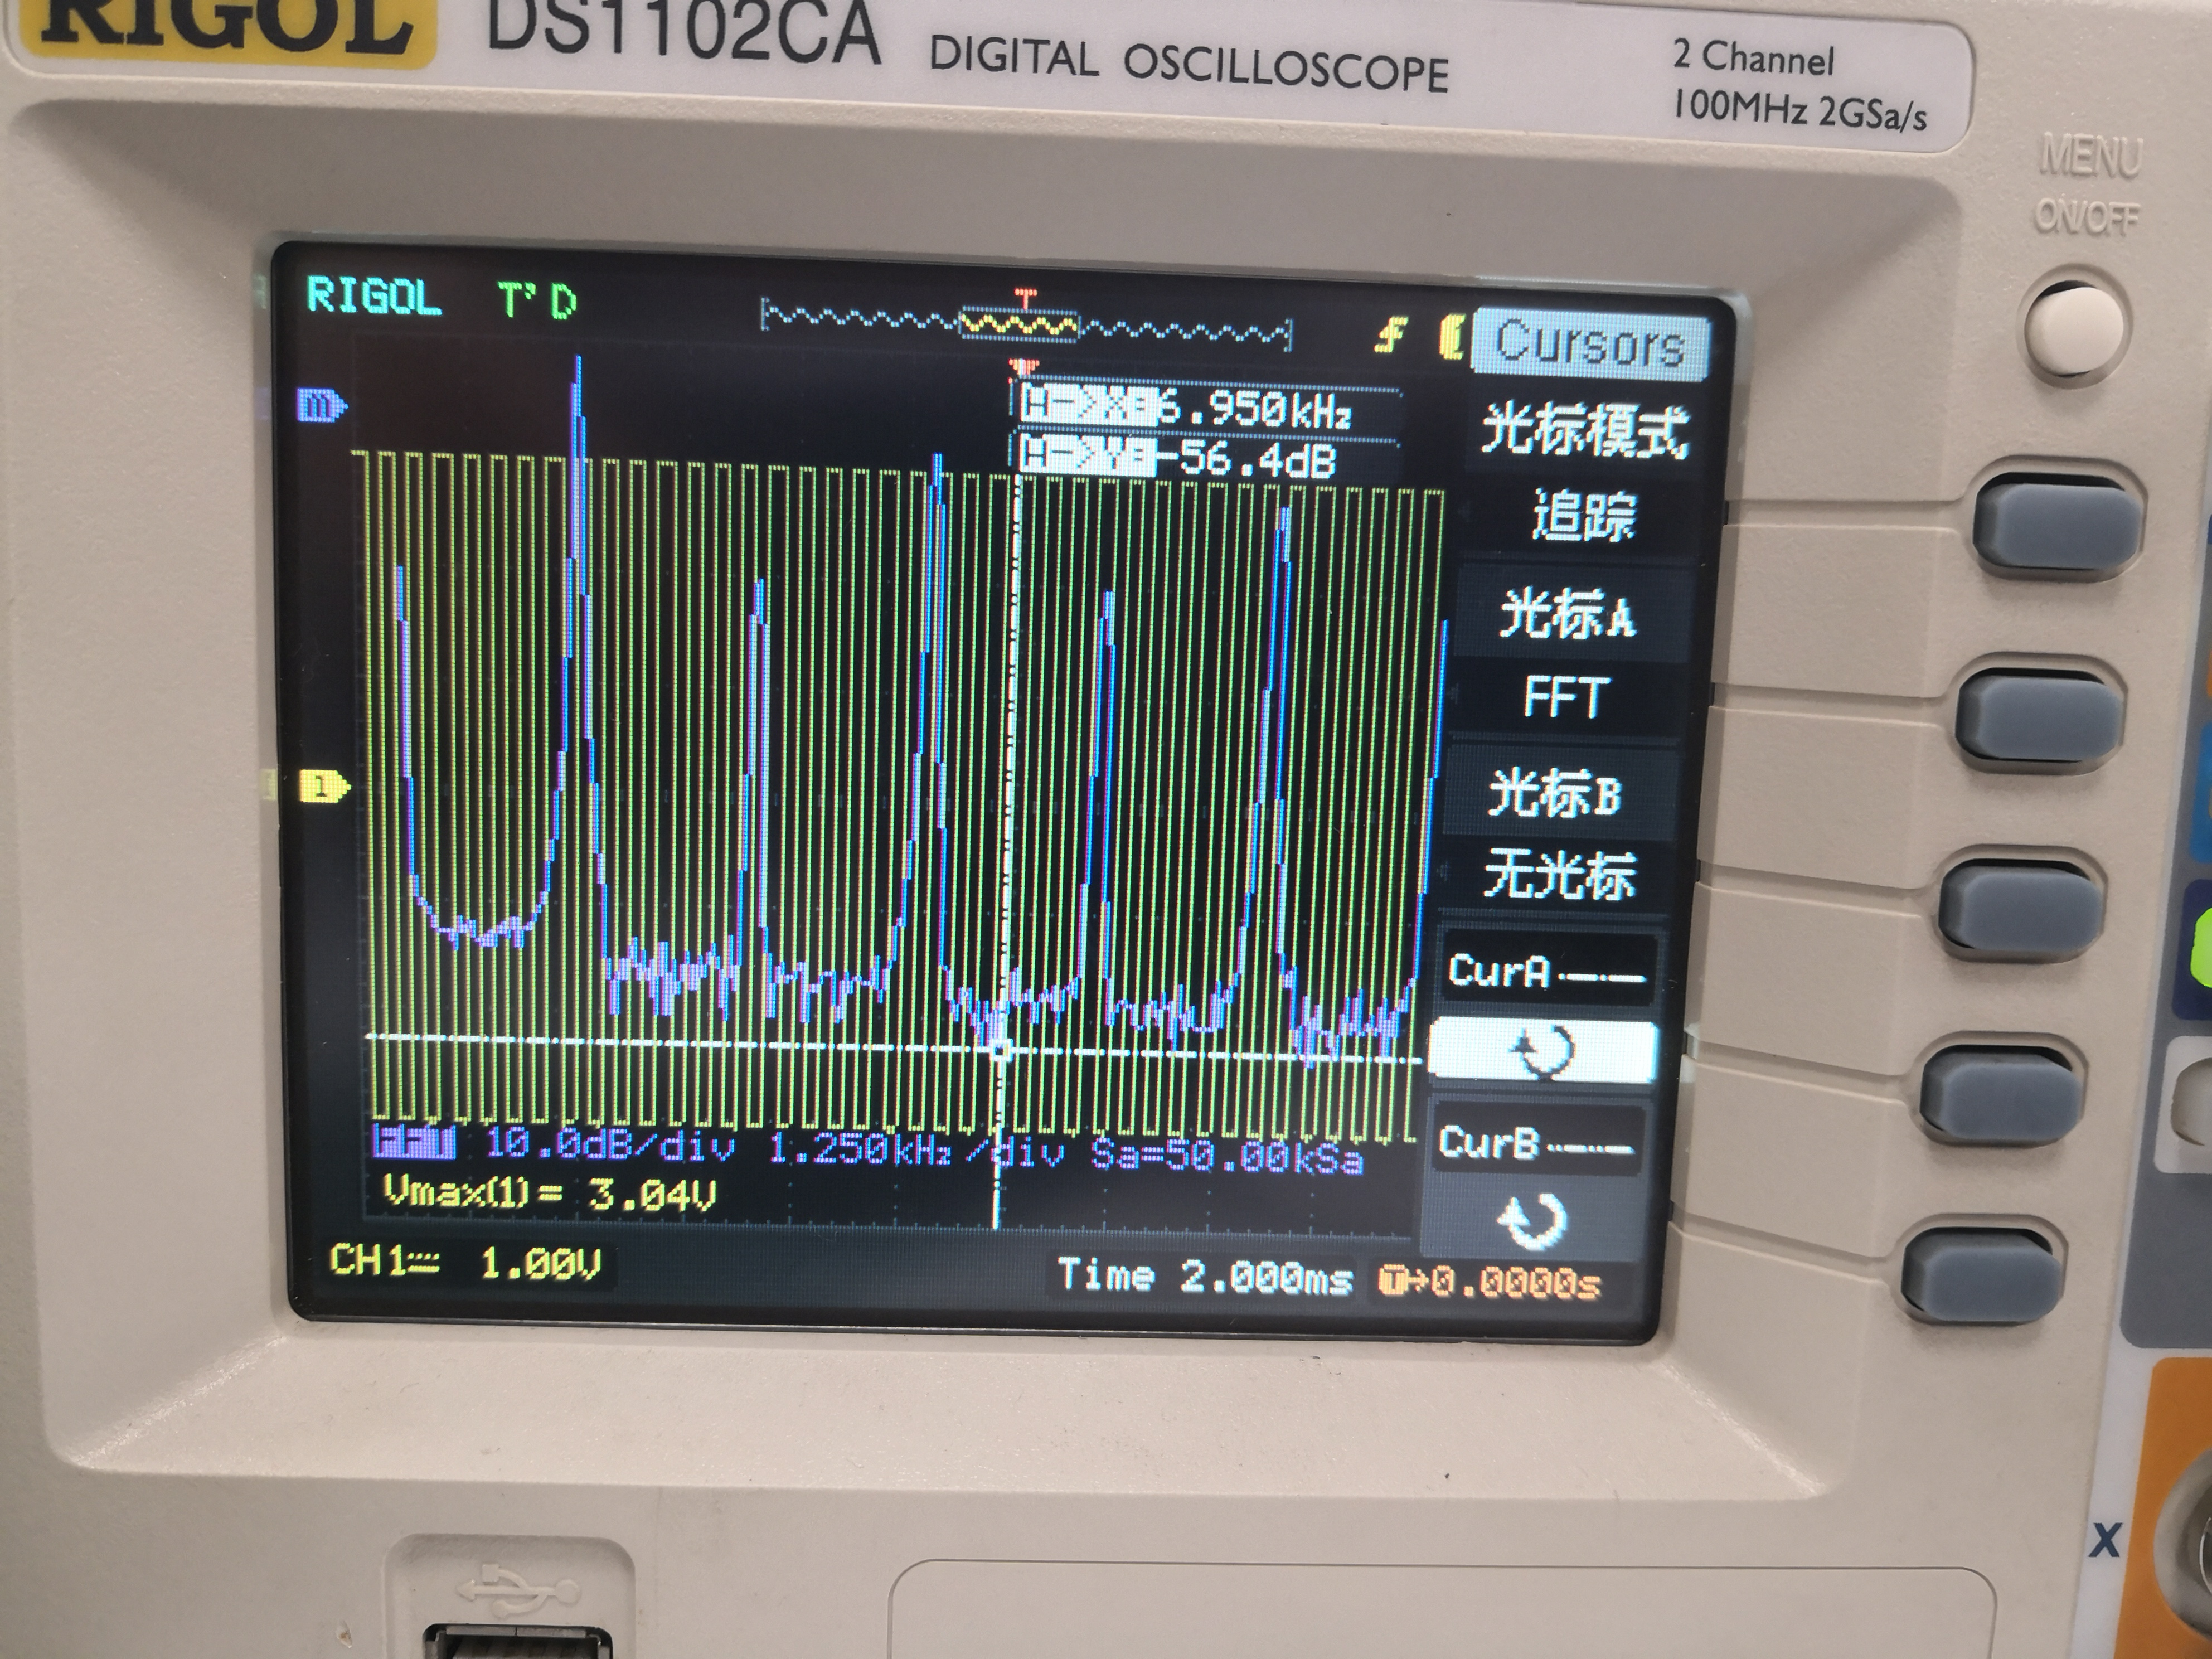
\includegraphics[width=0.45\textwidth]{5}
\end{figure}

\begin{figure}\centering
    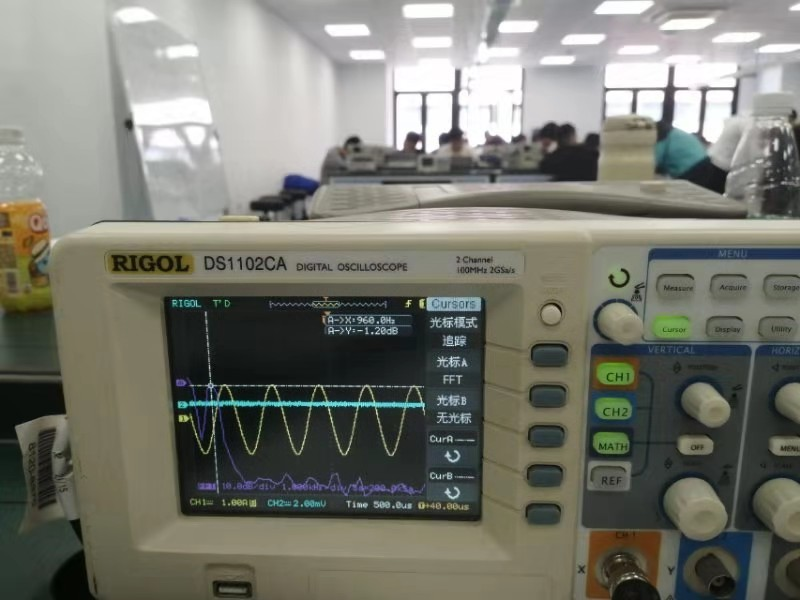
\includegraphics[width=0.45\textwidth]{6}
\end{figure}

\begin{figure}\centering
    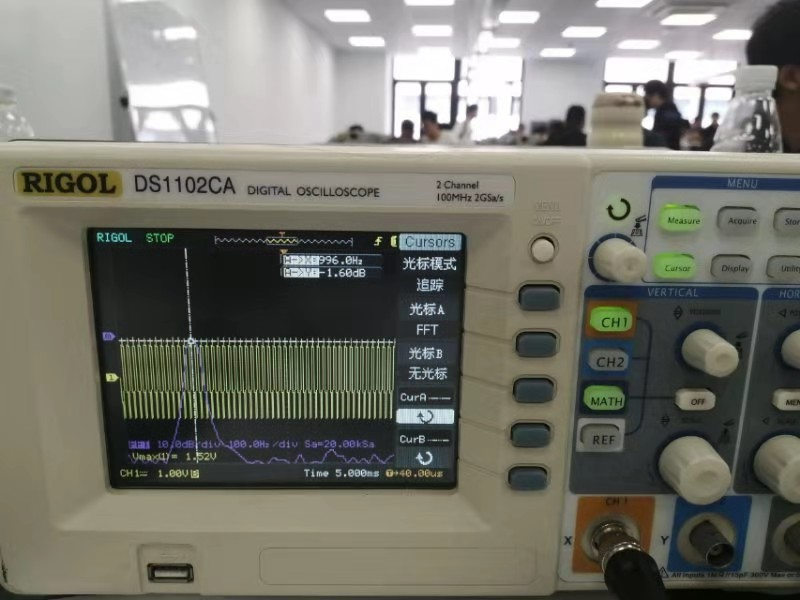
\includegraphics[width=0.45\textwidth]{7}
\end{figure}

\begin{figure}\centering
    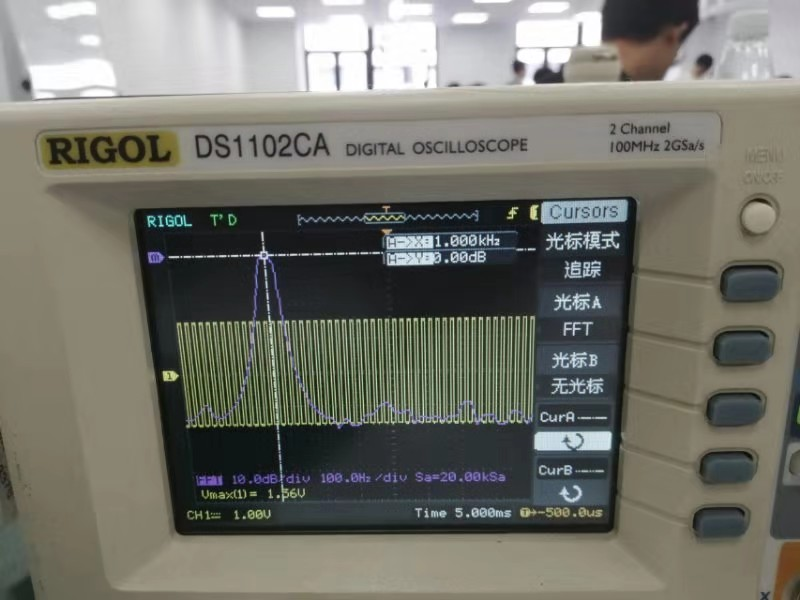
\includegraphics[width=0.45\textwidth]{8}
\end{figure}

\begin{figure}\centering
    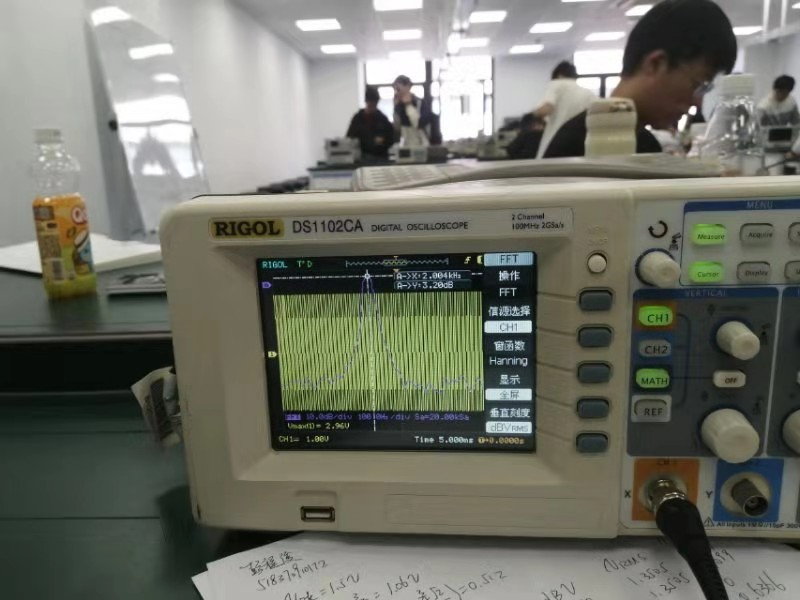
\includegraphics[width=0.45\textwidth]{9}
\end{figure}

\begin{figure}\centering
    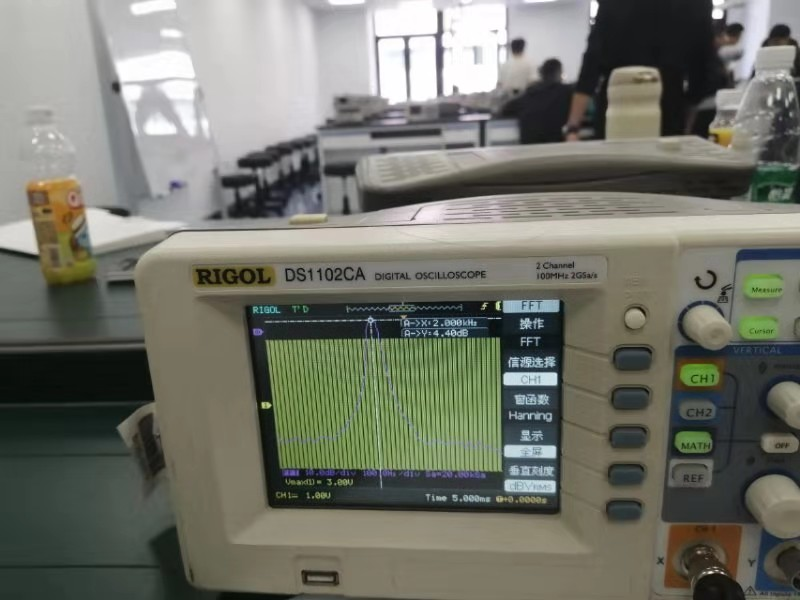
\includegraphics[width=0.45\textwidth]{10}
\end{figure}


\subsection{Data sheet}
The data sheet is attached at the end of the report.


\end{document}
